\documentclass{IMEKO2024}

%%%% Packages %%%%%%%%%%%%%%%%%%%%%%%%%%%%%%%%%%%%%%%%%%%%
\usepackage{amsmath}
\usepackage[colorlinks=true]{hyperref}
\usepackage{microtype}
\usepackage{proof}
\usepackage{mathtools}
\usepackage{graphicx}
\usepackage{rotating}
\usepackage{subcaption}
%\usepackage{multirow}
\usepackage{xkeyval}
\usepackage[font=small,justification=centering]{caption}
\captionsetup{labelsep = period}
\usepackage{subcaption}
\usepackage{floatrow}

%%%%%%%%%%%%%%%%%%%%%%%%%%%%%%%%%%%%%%%%%%%%%%%%%%%%%%%%%%

%%%% Macros %%%%%%%%%%%%%%%%%%%%%%%%%%%%%%%%%%%%%%%%%%%%%%
\newcommand{\pct}{\texttt{\symbol{37}}}
\newcommand{\dir}{\texttt{\symbol{62}}}
\newcommand{\res}{\texttt{\symbol{60}}}
\newcommand{\lcb}{\texttt{\symbol{123}}}
\newcommand{\rcb}{\texttt{\symbol{125}}}
\newcommand{\lsb}{\texttt{\symbol{91}}}
\newcommand{\rsb}{\texttt{\symbol{93}}}

\newcommand{\istype}[1]{#1\ \textsf{type}}
\newcommand{\isadd}[1]{#1\ \textsf{numeric}}
\newcommand{\ismult}[3]{(#1, #2, #3)\ \textsf{multipliable}}

\newcommand{\append}{+\!\!\!+}
\newcommand{\hjux}[2]{{#1}|{#2}}
\newcommand{\vjux}[2]{\frac{#1}{#2}}

\newcommand{\One}{\mathbf{1}}
\newcommand{\Matrix}[5]{\mathsf{Matrix}\,#1\,#2\,#3\,#4\,#5}
\newcommand{\List}[1]{\mathsf{List}\,#1}



\newcommand{\remph}{\emph}

\newcommand{\todo}[1]{\textcolor{red}{\textbf{TODO: #1}}}

%%%%%%%%%%%%%%%%%%%%%%%%%%%%%%%%%%%%%%%%%%%%%%%%%%%%%%%%%%

\begin{document}

\title{LabMate: supporting types for MATLAB}
\author{Conor McBride  \affiliationmark{1}, Georgi Nakov  \affiliationmark{1}, Fredrik Nordvall Forsberg  \affiliationmark{1}, Alistair Forbes  \affiliationmark{2}, Keith Lines  \affiliationmark{2}}
\affiliation{%
\affiliationmark{1}{\fontsize{11pt}{9pt} \selectfont University of Strathclyde , UK}  \\
\affiliationmark{2}{\fontsize{11pt}{9pt} \selectfont National Physical Laboratory, UK}}

\maketitle

\begin{abstract}
  TODO
\end{abstract}
\begin{keywords}
  TODO
\end{keywords}

\section{Introduction}

MATLAB is a key workhorse in many scientific and engineering
disciplines that are heavily reliant on numerical methods. It helps us
do powerful things. However, as with all software, MATLAB code may
contain implementation errors and bugs. In good programming practice
for MATLAB developers, programmers use comments to make clear what
physical systems their data concern and how the data should be
interpreted, specifying, e.g., units of measure for
quantities. Regrettably, none of this rich and often disciplined
metadata is perceptible to MATLAB, which instead enforces the
compatibility of producers and consumers of data by run-time checking
of tags which indicate only machine representation, not any form of
meaning. In reality, the programmers document meaning for each other's
benefit but keep the machine in the dark.

To rectify this situation, we have developed LabMate, which is a tool
to reify current virtuous engineering practices as a formal language
of MATLAB comments. MATLAB remains in the dark, but LabMate reads,
assesses, and transforms MATLAB programs in accordance with these
comments.
%
Behind the scenes, LabMate is retrofitting an expressive type system
to MATLAB, with the more of the meaning of programs recorded in their
types.
%
This gives a lightweight and low-cost way for MATLAB programmers to
express their intent, and in a language they are already working in,
rather than starting over from scratch.
%
While type systems and their theory is a well established discipline
of computer science, the development of LabMate has several novel
advances on the algebraic structure required to classify
matrices and the meanings of the quantities therein, e.g., their
physical dimensions. LabMate brings advanced type systems to
effectiveness within, rather than instead of, existing scientific and
engineering toolchains and practices.

\section{LabMate in action}
\label{sec:example}

% simple matrix multiplication example

The following greatly simplified, but still realistic, example from metrology  will help illustrate the principles of how LabMate will work. Consider one of the calculations required for measuring resistors using a cryogenic current comparator bridge~\cite{Williams_2010}.

An electrical current with a known value (the applied signal) is passed through the resistor being measured, and a series of voltage readings are taken at fixed time intervals (the recorded output). After a specified number of readings are taken, the direction of the input signal must be reversed in order to separate the offset and drift from the voltage readings. Therefore, the applied signal (bridge energisation) is a square wave of {\em reversals}. A calibration factor is also applied, dividing the signal into two parts with different amplitudes.

The recorded output follows the input signal, superimposed on a detector with noise, offset and drift. Figure~1%\ref{fig:rec_out}
provides an example of recorded output, using simulated data.
\begin{figure}[H]
  \begin{center}
    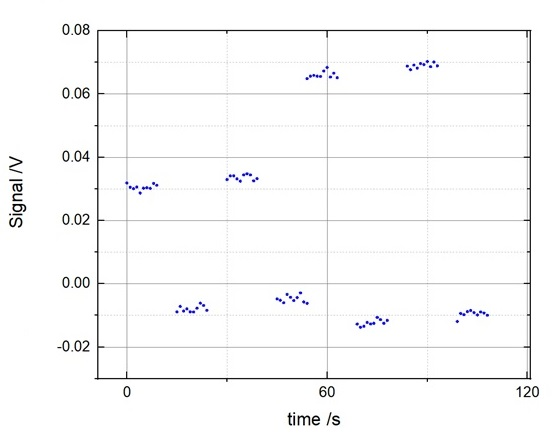
\includegraphics[width=0.6\linewidth]{example_output.jpg}
    \captionwide{Simulated example of recorded output.}
    \label{fig:rec_out}
  \end{center}
\end{figure}

The calculation of offset and drift is achieved using a least squares line fit calculated by solving a series of simultaneous equations, listed below. Note that although offset and drift differ for calibration and non-calibration parts of the input signal, the drift is the same in both cases.

% $t_i$ time ($\mathsf{T}$; in seconds); $v_i$ voltage ($\mathsf{ML}^2\mathsf{T}^{-3}\mathsf{I}^{-1}$; in volt)

\[
\begin{pmatrix*}
  d_{\textrm{nc}1} & d_{\textrm{c}1} & n_1 & c_1 & t_1  \\
  d_{\textrm{nc}2} & d_{\textrm{c}2} & n_2 & c_2 & t_2  \\
   & \vdots &  & & \\
  d_{\textrm{nc}N} & d_{\textrm{c}N} & n_N & c_N & t_N  \\
\end{pmatrix*}
\times
\begin{pmatrix}
  a \\
  a_{cal} \\
  c \\
  c_{cal} \\
  m
\end{pmatrix}
=
\begin{pmatrix}
  v_1 \\
  v_2 \\
  \vdots \\
  v_N
\end{pmatrix}
\]
%
The matrix on the left is made up of the following values:
%
\begin{itemize}
    \item The values in the first four columns are purely numeric and have no associated dimension.

    \item The first column will contain either $1$ or $-1$ for non-calibration voltage readings (i.e., those to which the calibration factor has not been applied) depending on the direction of the input signal. For calibration readings the value will be $0$.

    \item The second column contains equivalent values for voltage readings in which the calibration factor has been applied, i.e., $0$ for non-calibration readings and $1$ or $-1$ depending on the input signal direction for calibration readings.

    \item The third column contains $1$ for non-calibration readings and $0$ for calibration.

    \item The forth column is the opposite of the third.

    \item The fifth column contains time values.
\end{itemize}

The first row vector contains values to be calculated using the line fit. The second column vector contains voltage readings. The measured value of the resistor is calculated using the contents of the first row vector. Details of that calculation are beyond the scope of this paper.

This calculation can be converted into a MATLAB problem with LabMate annotations as follows, using MATLAB's builtin left division operator \texttt{A \textbackslash{} b} to compute a least squares fit. We then ask for the type of the resulting solution. Note that for reasons of space only twelve values are listed. A real measurement would contain considerably more values:
\begin{verbatim}
%> A :: [ 12 x 5 ] double
A = [ 1  0  1  0  t1
      1  0  1  0  t2
      1  0  1  0  t3
     -1  0  1  0  t4
     -1  0  1  0  t5
     -1  0  1  0  t6
      0  1  0  1  t7
      0  1  0  1  t8
      0  1  0  1  t9
      0 -1  0  1  t10
      0 -1  0  1  t11
      0 -1  0  1  t12 ]

%> b :: [ 12 x 1 ] double
b = [ v1 v2 v3 v4 v5 v6 ...
        v7 v8 v9 v10 v11 v12 ]

x = A \ b

%> typeof x
\end{verbatim}
%
The lines starting with `\texttt{\%>}' are interpreted as ordinary comments by MATLAB, but as \remph{input directives} by LabMate. LabMate acts by reading the source code and outputting it again, but possibly with some additional \remph{responses} to the directives added.

Did you notice the error in the above code? The vector \texttt{b} should be of size $12 \times 1$, but is erroneously of size $1 \times 12$ instead. LabMate detects this error and produces the following as output.
\begin{verbatim}
%> A :: [ 12 x 5 ] double
A = [ 1  0  1  0  t1
      1  0  1  0  t2
      1  0  1  0  t3
     -1  0  1  0  t4
     -1  0  1  0  t5
     -1  0  1  0  t6
      0  1  0  1  t7
      0  1  0  1  t8
      0  1  0  1  t9
      0 -1  0  1  t10
      0 -1  0  1  t11
      0 -1  0  1  t12 ]

%> b :: [ 12 x 1 ] double
%< unsolved constraints 12 =? 1, 1 =? 12
b = [ v1 v2 v3 v4 v5 v6 ...
        v7 v8 v9 v10 v11 v12 ]

x = A \ B

%> typeof x
%< the type of x is quite a puzzle
\end{verbatim}
%
That is, LabMate says that for \texttt{x} to have a sensible type, we need the (impossible) constraints $5 = 1$ and $1 = 5$ to be true, arising from the fact that we have declared \texttt{b} to be a $12 \times 1$ matrix, but in fact it is a $1 \times 12$ matrix. Note that the original source code has been retained exactly as is, including whitespace characters, but a response has been inserted to our \texttt{typeof} query. If we change \texttt{b} to
\begin{verbatim}
b = [ v1 v2 v3 v4 v5 v6 ...
        v7 v8 v9 v10 v11 v12 ]'
\end{verbatim}
using MATLAB's transpose operator instead, then LabMate responds
\begin{verbatim}
%< x :: [ 5 x 1 ] double
\end{verbatim}
This way, LabMate can detect matrix size errors at development time, rather than at runtime --- running the original code would indeed crash with the error \textcolor{red}{\textbf{\texttt{Matrix dimensions must agree}}}.

\section{Types for matrices}

Under the hood, LabMate translates MATLAB expressions to typed
expressions in its own core type theory.
%
Since matrices feature heavily in MATLAB code, the type of matrices
plays a central role in this type theory.
%
We make this type rather precise, by allowing the type of each entry
in the matrix to vary according to the row and column of the entry:
%
we parameterise the type of matrices by a type $R$ associated with
each row, a type $C$ associated with each column, and a type $E(x,y)$
which might vary depending on the values of parameters $x : R$ and
$y : C$, as well as two lists $rs : \List{R}$ and $\List{C}$ --- the
idea being that the $i$th entry in the list $rs$ and the $j$th entry
in the list $cs$ determines the type of the $(i, j)$ coordinate in the
matrix.
%
Matrix types formation can thus be summarised as the inference rule given in Figure~\ref{fig:matrix_intro}.
%\[
%  \infer{\istype{\Matrix{R}{C}{E}{rs}{cs}}}
%  {
%    \istype{R}
%    &\quad
%    \istype{C}
%    &\quad
%    x : R, y : C \vdash \istype{E(x,y)}
%    &\quad
%    rs : \List{R}
%    &\quad
%    cs : \List{C}
%  }
%\]
%
\begin{figure*}[th]
\begin{subfigure}{\textwidth}
  \begin{center}
    \[
      \infer{\istype{\Matrix{R}{C}{E}{rs}{cs}}}
      {
        \istype{R}
        &\quad
        \istype{C}
        &\quad
        x : R, y : C \vdash \istype{E(x,y)}
        &\quad
        rs : \List{R}
        &\quad
        cs : \List{C}
      }
    \]
  \end{center}
  \caption{Type formation rule for matrix types}
  \label{fig:matrix_intro}
\end{subfigure}
\hfill
\begin{subfigure}{\textwidth}
  \begin{center}
    \[
      \infer{A + B : \Matrix{R}{C}{E}{rs}{cs}}
      {
        x : R, y : C \vdash \isadd{E(x, y)}
        &\quad
        A : \Matrix{R}{C}{E}{rs}{cs}
        &\quad
        B : \Matrix{R}{C}{E}{rs}{cs}
      }
    \]
  \end{center}
  \caption{Addition rule for matrices}
  \label{fig:matrix_add}
\end{subfigure}
\hfill
\begin{subfigure}{\textwidth}
  \begin{center}
    \[
      \infer{A * B : \Matrix{R}{C}{E''}{rs}{cs}}
      {
        \ismult{E}{E'}{E''}
        &\quad
        A : \Matrix{R}{C}{E}{rs}{ms}
        &\quad
        B : \Matrix{R}{C}{E'}{ms}{cs}
      }
    \]
  \end{center}
  \caption{Multiplication rule for matrices}
  \label{fig:matrix_mul}
\end{subfigure}
% FIXME : \caption is broken
\captionwide{Typing rules for matrices}
\label{fig:matrix_rules}
\end{figure*}

A notable special case is when both $R$ and $C$ are the unit type
$R = C = \One$, that is, the type with exactly one element.
%
In this case, there is only one type of entries $E$ (because both $x$
and $y$ must be the unique element of the unit type), and the only
information available in the lists $rs : \List{\One}$ and
$cs : \List{\One}$ is their length.
%
Thus, we have recovered $\Matrix{\One}{\One}{E}{m}{n}$ as the type of
$m \times n$ matrices with entries of type $E$, where $n$ and $m$ are
the unique lists over the unit type of length $n$ and $m$
respectively.

Another noteworthy special case which we want to support takes $R$ and
$R$ to be types of physical dimensions, with $E(d_1, d_2)$ to be the
type of physical quantities of dimension $d_1 \cdot d_2^{-1}$.
%
This way, we can reduce dimensional consistency checking \`a la
Kennedy~\cite{kennedyUOM} also for programs involving matrices,
following the work of Hart~\cite{hart}.
%
We will see in Section~\ref{sec:example-revisited} how this can be helpful.

Terms of matrix type in the core type theory are built up from
$1 \times 1$ matrices and pasting matrices horizontally and vertically.
%
Singleton matrices have the following typing rule
\[
  \infer{[e] : \Matrix{R}{C}{E}{[r]}{[c]}}
    {r : R
      &\quad
      c : C
      &\quad
      e : E(r, c)
    }
\]
%
while horizontal and vertical pasting horizontally have the following
typing rules:
\[
  \infer{\hjux{A}{B} : \Matrix{R}{C}{E}{rs}{(cs_A \append cs_B)}}
  {
    A : \Matrix{R}{C}{E}{rs}{cs_A}
    &\quad
    B : \Matrix{R}{C}{E}{rs}{cs_B}
  }
\]
\[
  \infer{\vjux{A}{B} : \Matrix{R}{C}{E}{(rs_A \append rs_B)}{cs}}
  {
    A : \Matrix{R}{C}{E}{rs_A}{cs}
    &\quad
    B : \Matrix{R}{C}{E}{rs_B}{cs}
  }
\]
When comparing matrices for equality, we reassociate horizontal and
vertical pastings, so that $\hjux{\vjux{A}{C}}{\vjux{B}{D}}$ and
$\vjux{\hjux{A}{B}}{\hjux{C}{D}}$ indeed are considered equal.

The conditions for adding two matrices are given in Figure~\ref{fig:matrix_add} --- the matrices $A$ and $B$ can be added if all entry types $E(x, y)$ are
numeric (for example integers, or floating point numbers), and if $A$
and $B$ have the same matrix type.
%
%\[
%  \infer{A + B : \Matrix{R}{C}{E}{rs}{cs}}
%  {
%    x : R, y : C \vdash \isadd{E(x, y)}
%    &\quad
%    A : \Matrix{R}{C}{E}{rs}{cs}
%    &\quad
%    B : \Matrix{R}{C}{E}{rs}{cs}
%  }
%\]
%

Matrix multiplication is trickier, because it does not demand that $A$
and $B$ have the same type --- rather, it demands that $A$ and $B$
have \remph{compatible} types, see Figure~\ref{fig:matrix_mul}.
%
%\[
%  \infer{A * B : \Matrix{R}{C}{E''}{rs}{cs}}
%  {
%    \ismult{E}{E'}{E''}
%    &\quad
%    A : \Matrix{R}{C}{E}{rs}{ms}
%    &\quad
%    B : \Matrix{R}{C}{E'}{ms}{cs}
%  }
%\]
The entry types $E$, $E'$, $E''$ are multipliable if for all $x$, $y$
and $z$, we have that $E(x, y)$ and $E'(y, z)$ supports a
multiplication operation with codomain $E''(x, z)$.
%
This is certainly the case if all entry types involved are simply
integers or floating point numbers, but this constraint can also
ensure that the physical units involved line up.


% typechecking

\section{Implementation}

In contrast to most other typecheckers, LabMate works using a
\remph{transducer} model of interaction: it inputs MATLAB code with
formal comments, and outputs a new version of its input, responding to
the comments, as if it were a development collaborator.  It thus needs
to make sure that it retains as much of the input formatting as
possible.  Making sense of MATLAB code presented a significant reverse
engineering challenge, as the MATLAB syntax is largely specified
informally and by example.

LabMate elaborates MATLAB expressions and commands into terms of its own internal core type theory.
%
Because we want to ergonomically handle physical dimensions, matrices
and their types, this type theory has a richer equational theory than
other state-of-the-art type theories, which we achieve by a refined
normalisation algorithm for free Abelian groups, and free monoids.
%
The actual typechecking is implemented as a stack based virtual machine which uses unification and a limited form of backtracking to solve typing constraints.
%
After the virtual machine has solved as many problems as it can, we analyse its final state to reconstruct the output source code, perhaps with inserted warnings and error messages, or additional responses to queries.

LabMate is under constant development; the latest version can be found at \url{https://github.com/msp-strath/LabMate/tree/devel}.

\section{Supporting dimensional consistency}
\label{sec:example-revisited}

% matrix multiplication with units of measure

Coming back to the example from Section~\ref{sec:example} again, we can give both \texttt{A} and \texttt{B} more precise types, also taking their physical dimensions into account:
\begin{verbatim}
%> A :: [ i <- 12,  j <- 5 ]
          (if j == 4 then Q T else Q 1)

%> b :: [ 5 x 1 ] (Q (ML^2T^(-3)I^(-1)))
\end{verbatim}
This says that the entries in the last column of \texttt{A} are quantities of dimension time $\mathsf{T}$, while all other entries are dimensionless quantities. Meanwhile all the entries of \texttt{b} are quantities of dimension $\mathsf{ML}^{2}\mathsf{T}^{-3}\mathsf{I}^{-1}$. LabMate reports that the type of \texttt{x} should be
\begin{verbatim}
%< x :: [ i <- 5 ]
        (if i == 4
           then Q (ML^2T^(-4)I^(-1))
           else Q (ML^2T^(-3)I^(-1)))
\end{verbatim}
that is a $5 \times 1$ matrix whose entries are all quantities of dimension $\mathsf{ML}^{2}\mathsf{T}^{-3}\mathsf{I}^{-1}$ (i.e., units V) for entries in the first four rows and $\mathsf{ML}^{2}\mathsf{T}^{-4}\mathsf{I}^{-1}$ (i.e., units V/s) in the final row.
%
Another possible way to use LabMate is to instead declare that this is the expected type for \texttt{x}, and to leave the type of some of the entries in \texttt{b} as an unknown
\begin{verbatim}
%> b :: [ i <- 5 ]
        (if i == 4
           then ?bTy
           else Q (ML^2T^(-3)I^(-1)))
\end{verbatim}
We can then ask LabMate to solve the \remph{meta variable} \texttt{?bTy}, to which LabMate responds that we must also have \texttt{?aTy} = $\mathsf{Q}\,(\mathsf{ML}^{2}\mathsf{T}^{-3}\mathsf{I}^{-1})$. This way the types of LabMate can be used to validate and experiment with the dimensional consistency of the quantities involved.

%GravCalc example again: $t_i$ time ($\mathsf{T}$; in seconds); $v_i$ voltage ($\mathsf{ML}^2\mathsf{T}^{-3}\mathsf{I}^{-1}$; in volt)


\section{Conclusions and future work}

We have demonstrated how LabMate can help write MATLAB programs that are correct both in the sense that they avoid runtime errors, as well as dimensional inconsistency for physical dimensions.
%
Getting an error for types not matching can sometimes feel like a stick, but there are also plenty of opportunities for carrots, for example where the specification encoded in the type of the program admits a single unique solution, which could be generated automatically by LabMate.
%
Similarly, LabMate already has support for generating MATLAB code for serialising and deserialising complex data formats to and from files, based on a more high-level description of the data format (for example also taking units of measure into account)~\cite{mgen}.

So far, our focus has been on matrices, as this is what makes MATLAB
unique as a programming language.
%
In the future, we would like to also extend our coverage to
conditionals and loops, which might necessitate some approximation of
what is known about program fragments at runtime.

\section{Acknowledgements}

This work was undertaken jointly by the Mathematically Structured Programming Group of the University of Strathclyde and the National Physical Laboratory’s Data Science department as part of Data Science’s Tools for Trustworthiness National Measurement System (NMS) project 2023 – 2024.

Thanks to NPL colleague Nick Fletcher for his help and guidance providing the example from Section \ref{sec:example}. Thanks also to NPL colleagues Louise Wright and Ian Smith for reviewing this paper, and to Professor Neil Ghani for his support.

\bibliographystyle{ws-procs9x6}
\bibliography{labmate}
%\printbibliography
\end{document}

%%% Local Variables:
%%% mode: latex
%%% TeX-master: t
%%% End:
